\documentclass[aspectratio=169]{beamer}

\usepackage{ctex}
\usepackage{amsmath,amsfonts,amssymb,bm}
\usepackage{graphicx}
\usepackage{booktabs}
\usepackage{tabularx}
\usepackage{array}
\usepackage{ragged2e}
\usepackage{hyperref}
\usepackage{pgfpages}
\usepackage{xcolor}

\usetheme{Berlin}
\usecolortheme{whale}
\useinnertheme[shadow=true]{rounded}
\usefonttheme[onlymath]{serif}
\setbeamercovered{transparent}
\setbeamertemplate{navigation symbols}{}
\hypersetup{hidelinks}

\newcolumntype{Y}{>{\RaggedRight\arraybackslash}X}
\newcommand{\best}[1]{\textbf{\color{blue!65!black}#1}}
\newcommand{\warn}[1]{\textbf{\color{red!70!black}#1}}
\newcommand{\source}[1]{\par\vspace{1mm}{\tiny\color{black!60}来源：#1}}
\newcommand{\eqtagtext}[1]{\qquad\text{#1}}

\graphicspath{{artifacts/diffusion_physics_group_meeting/sources/pfgmpp_source/img/}{artifacts/diffusion_physics_group_meeting/sources/speed_accuracy_source/figures/}{figures/physics_diffusion_group_meeting/}}

\makeatletter
\newif\ifpympressnotesright
\newif\ifpympressnotesafter
\@ifundefined{pympressnotesright}{\pympressnotesrightfalse}{\pympressnotesrighttrue}
\@ifundefined{pympressnotesafter}{\pympressnotesafterfalse}{\pympressnotesaftertrue}
\makeatother
\ifpympressnotesright
  \setbeameroption{show notes on second screen=right}
\else\ifpympressnotesafter
  \setbeameroption{show notes}
\else
  \setbeameroption{hide notes}
\fi\fi
\newcommand{\speakernote}[1]{\note{\footnotesize #1}}

\setbeamertemplate{footline}{%
 \leavevmode%
 \hbox{%
 \begin{beamercolorbox}[wd=.31\paperwidth,ht=2.25ex,dp=1ex,center]{author in head/foot}
 \insertshortauthor
 \end{beamercolorbox}%
 \begin{beamercolorbox}[wd=.38\paperwidth,ht=2.25ex,dp=1ex,center]{title in head/foot}
 \insertshorttitle
 \end{beamercolorbox}%
 \begin{beamercolorbox}[wd=.31\paperwidth,ht=2.25ex,dp=1ex,center]{date in head/foot}
 \insertshortdate \quad \insertframenumber/\inserttotalframenumber
 \end{beamercolorbox}%
 }
}

\title[物理启发的扩散模型]{理论物理如何重写扩散模型的加噪与去噪？}
\subtitle{Poisson 电场、非平衡热力学与最优传输}
\author[刘嘉瑞]{汇报人：刘嘉瑞}
\institute[论文组会]{近年论文阅读汇报\\PFGM++（ICML 2023）与 Speed--Accuracy Relations（PRX 2025）}
\date{2026年8月30日}

\begin{document}

% 1
\begin{frame}
  \titlepage
  \speakernote{老师好，我这一个月主要沿着一个问题看了两篇论文：扩散模型里的加噪和去噪，能不能不只靠经验设计，而是直接从理论物理方程出发。第一篇 PFGM++ 用的是电静力学里的 Poisson 场，重点改造从噪声回到数据的生成轨迹；第二篇是 2025 年发表在 Physical Review X 的工作，用非平衡热力学和最优传输分析噪声日程。今天我想讲清楚的主线是：物理规律到底进入了模型的哪一步，以及它带来了什么可验证的好处。}
\end{frame}

% 2
\begin{frame}{我为什么选这两篇？}
\small
\begin{block}{同一个问题，两种互补回答}
\centering
\best{怎样让“加噪--去噪”不再只是经验工程？}
\end{block}

\vspace{1mm}
\begin{columns}[T,onlytextwidth]
\begin{column}{0.49\textwidth}
\begin{alertblock}{论文 1：重写生成轨迹}
\textbf{PFGM++}（ICML 2023）
\begin{itemize}
  \item 把数据看成电荷。
  \item 用高维 Poisson 电场线连接先验与数据。
  \item 用维数 $D$ 调节鲁棒性与学习难度。
\end{itemize}
\end{alertblock}
\end{column}
\begin{column}{0.49\textwidth}
\begin{exampleblock}{论文 2：重写噪声日程准则}
\textbf{Speed--Accuracy Relations}（PRX 2025）
\begin{itemize}
  \item 把前向扩散视为耗散过程。
  \item 用熵产生约束生成误差。
  \item 用 Wasserstein 测地线给出最优路径。
\end{itemize}
\end{exampleblock}
\end{column}
\end{columns}

\vspace{1mm}
\begin{center}
\large 一篇偏\best{模型构造}，一篇偏\best{理论边界}。
\end{center}
\speakernote{我没有选那种只在最终损失里加一个物理约束的应用论文，因为那类工作通常是在约束生成结果，而不是改造一般扩散模型本身。这里两篇正好互补：PFGM++ 直接换掉生成路径的物理几何；PRX 这篇则告诉我们，前向加噪走得多快、走哪条路，会怎样影响反向生成的误差上界。所以它们分别回答“怎么走”和“为什么这样走更好”。}
\end{frame}

% 3
\begin{frame}{先统一语言：普通扩散模型在做什么？}
\small
\begin{columns}[T,onlytextwidth]
\begin{column}{0.47\textwidth}
\begin{block}{前向：逐步加噪}
\[
\bm{x}_t=m_t\bm{x}_0+\sigma_t\bm{\epsilon},
\qquad \bm{\epsilon}\sim\mathcal N(\bm 0,\bm I)
\]
\begin{itemize}
  \item $m_t$：保留多少信号；
  \item $\sigma_t$：加入多少噪声；
  \item 两者随时间的变化就是\best{noise schedule}。
\end{itemize}
\end{block}
\end{column}
\begin{column}{0.51\textwidth}
\begin{block}{反向：估计 score，再积分回去}
\[
\frac{d\bm{x}}{dt}
=-\dot\sigma(t)\sigma(t)
\nabla_{\bm{x}}\log p_{\sigma(t)}(\bm{x})
\]
\begin{itemize}
  \item 网络学习不同噪声强度下的 score；
  \item 采样器沿 ODE/SDE 多步去噪；
  \item 误差来自网络估计与数值离散。
\end{itemize}
\end{block}
\end{column}
\end{columns}

\begin{alertblock}{两篇论文分别动了哪里？}
PFGM++ 改造\best{扰动核和反向轨迹}；PRX 论文给\best{前向噪声路径}建立物理优化准则。
\end{alertblock}
\speakernote{先用这一页统一符号。最常见的连续扩散可以写成 x\_t 等于衰减后的干净数据加高斯噪声。m\_t 和 sigma\_t 随时间怎么变，就是噪声日程。反向时，网络估计 score，也就是对数密度的梯度，然后通过 ODE 或 SDE 一步步回到数据。这里要记住两个误差来源：第一是网络没有把向量场学准，第二是有限步数积分会产生离散误差。接下来 PFGM++ 主要改向量场的物理来源，第二篇主要研究噪声日程走得快不快。}
\end{frame}

\section{PFGM++：Poisson 电场驱动生成}

% 4

\begin{frame}{论文 1：PFGM++ 的一句话思想}
\scriptsize
\begin{block}{Xu et al., ICML 2023\\[-1mm]
\textbf{PFGM++: Unlocking the Potential of Physics-Inspired Generative Models}}
\end{block}

\begin{columns}[T,onlytextwidth]
\begin{column}{0.47\textwidth}
\begin{alertblock}{普通扩散}
把数据逐渐搅成高斯噪声，再学习如何逆转。
\end{alertblock}
\end{column}
\begin{column}{0.51\textwidth}
\begin{exampleblock}{PFGM++}
把数据点放在高维“地面”上当正电荷，从远处沿\best{电场线}回到数据分布。
\end{exampleblock}
\end{column}
\end{columns}

\begin{center}
\large 数据分布 $\longleftrightarrow$ 电荷分布，\quad
生成轨迹 $\longleftrightarrow$ 电场线
\end{center}

\begin{block}{统一视角}
原始 PFGM 加 1 个维度；PFGM++ 加 $D$ 个维度：
\[
D=1\Rightarrow\text{PFGM},\qquad D\to\infty\Rightarrow\text{扩散模型}.
\]
\end{block}
\speakernote{第一篇的核心类比是：普通扩散先把数据搅成噪声，再学反向场；PFGM++ 把数据当作高维空间里的正电荷，沿电场线从远处回到数据。它把原始 PFGM 和扩散模型统一到增广维数 D：D 等于 1 是 PFGM，D 趋于无穷恢复 diffusion。}
\end{frame}

% 5

\begin{frame}{物理公式如何变成去噪轨迹？}
\scriptsize
\begin{columns}[T,onlytextwidth]
\begin{column}{0.54\textwidth}
\begin{block}{高维库仑场}
令 $\tilde{\bm{x}}=(\bm{x},\bm{z})\in\mathbb R^{N+D}$，数据位于 $\bm z=0$：
\[
\bm E(\tilde{\bm x})=
\frac{1}{S_{N+D-1}(1)}\int
\frac{\tilde{\bm x}-\tilde{\bm y}}
{\lVert\tilde{\bm x}-\tilde{\bm y}\rVert^{N+D}}p(\bm y)d\bm y.
\]
\end{block}
\begin{alertblock}{旋转对称带来的降维}
$D$ 个增广坐标只需保留半径
\[
r=\lVert\bm z\rVert_2,\qquad
\frac{d\bm x}{dr}=\frac{\bm E_x}{E_r}.
\]
\end{alertblock}
\end{column}
\begin{column}{0.44\textwidth}
\centering
\includegraphics[height=0.54\textheight]{D_illustration.png}
\\[-1mm]
{\tiny\color{black!60}Xu et al., 2023, Fig. 1}
\end{column}
\end{columns}
\speakernote{这一页是物理核心。作者把 N 维数据扩展到 N 加 D 维，电场由高维库仑定律给出。由于增广坐标有旋转对称性，D 个坐标不用逐个跟踪，只保留长度 r。于是生成轨迹就是横向电场除以径向电场，r 从大降到 0 时，样本沿电场线落回数据平面。}
\end{frame}

% 6


\begin{frame}{怎样训练网络学到这个电场？\hfill{\footnotesize（时间紧可略讲）}}
\scriptsize
\begin{block}{物理诱导的扰动核}
对干净样本 $\bm y$，在半径 $r$ 处采样 $\bm x$：
\[
p_r(\bm x\mid\bm y)\propto
\bigl(\lVert\bm x-\bm y\rVert_2^2+r^2\bigr)^{-(N+D)/2}.
\]
幂次来自高维库仑场，因此平方损失的最优解与电场\best{方向一致}。
\end{block}

\begin{block}{可训练目标与采样}
\[
\mathcal L=\mathbb E\left[\left\lVert f_\theta(\bm x,r)-
\frac{\bm x-\bm y}{r/\sqrt D}\right\rVert_2^2\right],
\qquad
\frac{d\bm x}{dr}=\frac{f_\theta(\bm x,r)}{\sqrt D}.
\]
从大 $r$ 积分到 $r=0$。
\end{block}

\vspace{-1mm}
{\scriptsize\color{red!70!black}\textbf{工程收益：}不需要原始 PFGM 的大 batch 电场近似；单样本条件生成也能训练。}
\speakernote{作者不直接对整个数据集求电场积分，而是设计一个幂次来自库仑定律的重尾扰动核。这样平方损失的最优输出会和真实电场方向一致。训练目标和扩散模型的去噪匹配相似，训练后把 r 从大到小积分；同时省掉原始 PFGM 的大 batch 近似。}
\end{frame}

% 7


\begin{frame}{$D$ 为什么是关键旋钮？}
\scriptsize
\begin{columns}[T,onlytextwidth]
\begin{column}{0.48\textwidth}
\begin{block}{理论极限}
令 $r=\sigma\sqrt D$。当 $D\to\infty$ 时，
\[
-\frac{\sqrt D\,\bm E_x}{E_r}
\longrightarrow \sigma\nabla_{\bm x}\log p_\sigma(\bm x),
\]
所以 PFGM++ 恢复 diffusion probability-flow ODE。
\end{block}
\end{column}
\begin{column}{0.50\textwidth}
\begin{alertblock}{有限 $D$ 的权衡}
\begin{itemize}
  \item $D$ 大：半径更集中、易拟合，但轨迹偏离时更脆弱；
  \item $D$ 小：重尾更宽、抗误差和大步长，但更难学；
  \item 甜点区通常在 $(1,\infty)$ 中间。
\end{itemize}
\end{alertblock}
\end{column}
\end{columns}

\vspace{-2mm}
\begin{center}
\includegraphics[height=1.45cm]{p_r_D.pdf}
\\[-1mm]
{\tiny\color{black!60}扰动半径随 $D$ 增大而集中（Xu et al., 2023）。}
\end{center}
\speakernote{D 是控制鲁棒性和刚性的旋钮。D 趋于无穷时，重尾扰动变成高斯，电场方向变成 score，ODE 回到扩散模型。有限 D 的扰动更宽，采样轨迹跑偏时更容易被拉回，但也更难学习，所以最佳点通常在中间。}
\end{frame}

% 8

\begin{frame}{PFGM++ 的结果：更好，还是只是更“物理”？}
\scriptsize
\begin{columns}[T,onlytextwidth]
\begin{column}{0.51\textwidth}
\centering
\includegraphics[width=0.90\linewidth]{alpha_fid_cifar.pdf}
\\[-1mm]
{\tiny\color{black!60}Xu et al., 2023：CIFAR-10 轨迹扰动实验}
\end{column}
\begin{column}{0.47\textwidth}
\begin{block}{论文报告}
\begin{itemize}
  \item 有限 $D$ 在 CIFAR-10、FFHQ 64、LSUN Churches 256 上超过当时强扩散基线；
  \item CIFAR-10 类条件设置：$D=2048$，FID $=1.74$；
  \item 小 $D$ 对轨迹噪声、量化误差和少采样步更鲁棒。
\end{itemize}
\end{block}
\begin{alertblock}{我的判断}
贡献不是“电场永远更好”，而是揭示了\best{拟合难度--采样鲁棒性}的结构性权衡。
\end{alertblock}
\end{column}
\end{columns}
\speakernote{左图给每个 ODE 步加入轨迹误差，alpha 越大表示偏得越多。普通扩散，也就是 D 趋于无穷，FID 很快恶化；D 等于 64 或 128 的退化慢得多。论文还报告多个图像数据集上的强结果和 CIFAR-10 类条件 FID 1.74。我的判断是，重点不是某个单点数字，而是它给出了一个可调模型族。}
\end{frame}

\section{PRX 2025：非平衡热力学优化噪声路径}

% 9
\begin{frame}{论文 2：把前向加噪看成耗散过程}
\footnotesize
\begin{block}{Ikeda et al., Physical Review X 15, 031031 (2025)}
\textbf{Speed--Accuracy Relations for Diffusion Models: Wisdom from Nonequilibrium Thermodynamics and Optimal Transport}
\end{block}

\begin{columns}[T,onlytextwidth]
\begin{column}{0.52\textwidth}
\begin{block}{Fokker--Planck / Langevin 表述}
\[
\partial_t P_t
=-\nabla\!\cdot(\bm\nu_t^P P_t),
\qquad
\bm\nu_t^P=\bm f_t-T_t\nabla\log P_t,
\]
\[
d\bm x_t=\bm f_t(\bm x_t)dt+\sqrt{2T_t}\,dB_t.
\]
\end{block}
\end{column}
\begin{column}{0.46\textwidth}
\begin{alertblock}{物理量翻译}
\begin{itemize}
  \item $T_t$：布朗粒子的温度 $\leftrightarrow$ 噪声强度；
  \item $\bm f_t$：外力 $\leftrightarrow$ 漂移项；
  \item $\bm\nu_t^P$：概率密度在分布空间里的速度；
  \item 前向扩散：不可逆、产生熵的耗散过程。
\end{itemize}
\end{alertblock}
\end{column}
\end{columns}

\begin{center}
\large 核心问题：\best{前向分布移动得太快，会不会放大反向生成误差？}
\end{center}
{\tiny\color{black!60}Ikeda et al., Physical Review X 15, 031031 (2025)}
\speakernote{第二篇从 Fokker--Planck 方程重新看扩散模型。P\_t 是数据分布随时间的变化，nu 是分布流动的速度场。等价的 Langevin 方程里，T\_t 可以理解成温度，也就是噪声强度，f\_t 是外力或漂移。这样一来，前向加噪就是一个布朗粒子的非平衡耗散过程，会产生熵。作者关心的不是再设计一个更大的网络，而是问：如果前向分布在 Wasserstein 空间里移动得太快，反向过程起点的一点小误差，会不会被放大成最终生成误差？}
\end{frame}

% 10
\begin{frame}{热力学量：熵产生就是“走这条扩散路径的代价”}
\small
\begin{block}{熵产生率}
\[
\dot S_t^{\mathrm{tot}}
=
\frac{1}{T_t}
\int
\lVert\bm\nu_t^P(\bm x)\rVert_2^2
P_t(\bm x)d\bm x
\ge 0.
\]
\end{block}

\begin{columns}[T,onlytextwidth]
\begin{column}{0.48\textwidth}
\begin{exampleblock}{物理解释}
分布移动得越快、速度场越强，单位时间耗散越大；非负性对应热力学第二定律。
\end{exampleblock}
\end{column}
\begin{column}{0.50\textwidth}
\begin{alertblock}{机器学习解释}
前向过程不是只看起点和终点：\best{中间路径}也决定反向生成对初始误差有多敏感。
\end{alertblock}
\end{column}
\end{columns}

\vspace{2mm}
当外力是保守力时，
\[
T_t\dot S_t^{\mathrm{tot}}=[v_2(t)]^2,
\]
其中 $v_2(t)$ 是分布在 $2$-Wasserstein 空间中的瞬时速度。
\speakernote{作者用熵产生率衡量这条前向扩散路径的耗散。这个公式本质上是速度场平方的期望，再除以温度，所以分布移动越剧烈，熵产生越大。它非负，对应第二定律。机器学习上的关键翻译是：即使前向过程的起点都是数据、终点都是高斯，不同的中间路径也不是等价的。保守力情况下，温度乘熵产生率正好等于二阶 Wasserstein 空间里的速度平方，所以我们可以不用真的测物理热量，而是直接用分布移动速度来讨论噪声日程。}
\end{frame}

% 11

\begin{frame}{核心定理：扩散越“急”，生成误差上界越大}
\footnotesize
\begin{columns}[T,onlytextwidth]
\begin{column}{0.46\textwidth}
\centering
\includegraphics[width=0.92\linewidth]{SADMconcept.pdf}
\\[-1mm]
{\tiny\color{black!60}Ikeda et al., 2025, Fig. 5}
\end{column}
\begin{column}{0.52\textwidth}
\begin{block}{速度--精度关系}
\[
\boxed{\displaystyle
\frac{(\Delta W_1)^2}{\tau D_0}
\le \int_0^\tau [v_2(t)]^2dt}
\]
\end{block}
\begin{itemize}
  \item $D_0$：实际先验与真实反向起点的偏差；
  \item $\Delta W_1$：该偏差造成的最终分布误差变化；
  \item 右侧：前向路径的\best{扩散速度代价}。
\end{itemize}
\begin{alertblock}{一句话}
前向路径越急、耗散越大，反向结果的最坏敏感性越高。
\end{alertblock}
\end{column}
\end{columns}
\speakernote{这是第二篇最重要的式子。D\_0 是实际采样先验和真实反向起点的初始偏差，Delta W\_1 是它经过反向过程后造成的误差变化，右边是前向分布速度平方的积分。结论是前向路径的速度代价控制误差响应上界。不是说速度大必然失败，而是说最坏敏感性会变大，所以低耗散路径更有鲁棒性保证。}
\end{frame}

% 12

\begin{frame}{怎样得到更好的 noise schedule？走 Wasserstein 测地线}
\footnotesize
\begin{block}{固定起点、终点和总时长 $\tau$}
\[
\int_0^\tau [v_2(t)]^2dt
\ge \frac{W_2^2(P_0,P_\tau)}{\tau}.
\]
等号成立时，$P_t$ 沿 $2$-Wasserstein 测地线匀速前进：
\[
v_2(t)=\frac{W_2(P_0,P_\tau)}{\tau}.
\]
\end{block}

\begin{columns}[T,onlytextwidth]
\begin{column}{0.48\textwidth}
\begin{exampleblock}{直觉}
像搬沙子：每份概率质量走最短、最均匀的路线，避免前面猛冲、后面补救。
\end{exampleblock}
\end{column}
\begin{column}{0.50\textwidth}
\begin{alertblock}{对已有日程的解释}
\begin{itemize}
  \item cond-OT / flow matching：条件层面的近似 OT；
  \item cosine：较平滑，但一般不是全局测地线；
  \item 真正 OT：代价最低，但高维构造更贵。
\end{itemize}
\end{alertblock}
\end{column}
\end{columns}
\speakernote{有了误差上界后，优化目标就是降低扩散速度代价。固定起点、终点和总时间时，最小代价对应 Wasserstein 测地线，而且要匀速走。直觉上像搬沙子，不要一开始把结构冲散，再在后面补救。cond-OT 可以看成条件分布层面的可计算近似，但真实高维 OT 仍然昂贵，所以这篇主要提供设计准则。}
\end{frame}

% 13


\begin{frame}{数值证据：OT 路径更慢地破坏结构，也更容易反演}
\tiny
\begin{columns}[T,onlytextwidth]
\begin{column}{0.64\textwidth}
\centering
\includegraphics[width=0.86\linewidth]{swiss_roll_with_process_light.pdf}
\end{column}
\begin{column}{0.34\textwidth}
\begin{block}{读图}
蓝色是前向加噪，粉色是估计反向；从左到右为 $t/\tau$ 增大。OT 在中间时刻保留螺旋结构更久。
\end{block}
\begin{alertblock}{验证}
多种初始扰动下不等式成立；OT 的误差响应 $\eta$ 最小；在 CelebA-HQ、LSUN bedroom 潜空间中也能估计上界。
\end{alertblock}
\end{column}
\end{columns}
\speakernote{这个图最直观。cosine 很早就把螺旋结构搅散，cond-OT 好一些，而真正 OT 在中间阶段保留结构最久，所以更容易反演。作者还验证了不同初始偏差下的不等式，并在两个真实图像数据集的潜空间中估计上界。要注意，这主要是理论关系的数值验证，不等于低成本替换所有大模型日程的算法。}
\end{frame}

\section{对比与总结}

% 14
\begin{frame}{两篇论文放在一起：物理到底优化了什么？}
\scriptsize
\centering
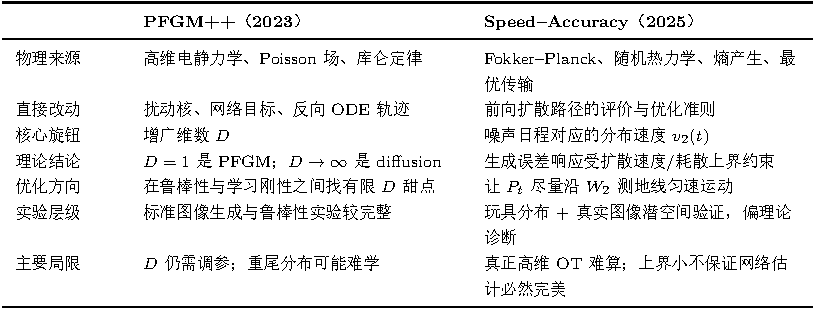
\includegraphics[width=0.92\linewidth]{comparison_table.pdf}

\vspace{-1mm}
\begin{alertblock}{我的综合理解}
物理规律最有价值的地方，不是给模型贴“可解释”标签，而是把经验选择变成\best{可推导的向量场、可调参数和可比较的代价函数}。
\end{alertblock}
\speakernote{把两篇放在一起看，PFGM++ 更像一个可以直接训练和采样的新模型族，它回答反向轨迹怎么构造；PRX 论文更像理论标尺，回答什么样的前向路径对误差更稳。它们共同说明，物理的价值不只是类比，而是把经验组件变成可推导对象：PFGM++ 给出电场向量场和 D 这个结构参数；PRX 给出熵产生、Wasserstein 速度和误差上界。两篇也都有局限：PFGM++ 需要调 D，PRX 的真实高维最优传输很难算，而且理论上界不能替代网络本身的拟合质量。}
\end{frame}

% 15
\begin{frame}{结论：我这个月得到的三个认识}
\small
\begin{enumerate}
  \item \textbf{加噪分布不一定非得是高斯。}\\
  PFGM++ 用 Poisson 场诱导的重尾扰动，把扩散模型放进更大的物理模型族。
  \item \textbf{去噪误差不只由网络大小决定。}\\
  轨迹是否覆盖模型误差、数值步长是否把样本带离训练区域，同样决定鲁棒性。
  \item \textbf{noise schedule 本质上是分布空间中的路径规划。}\\
  非平衡热力学表明，路径过快、耗散过大，会抬高反向误差敏感性的上界；$W_2$ 测地线提供理论最优标尺。
\end{enumerate}

\begin{alertblock}{可以继续追的问题}
能否把有限 $D$ 的 Poisson 路径与近似 Wasserstein 测地线结合，既获得 PFGM++ 的抗误差能力，又降低前向扩散速度代价？
\end{alertblock}

\vfill
\begin{center}
\Large 谢谢老师，请批评指正。
\end{center}
\speakernote{最后总结三点。第一，高斯加噪只是扩散模型的一种选择，PFGM++ 证明重尾、物理诱导的扰动也可以形成严格生成模型。第二，采样质量不只取决于网络预测准不准，还取决于轨迹本身对误差和步长是否鲁棒。第三，噪声日程可以看成分布空间里的路径规划，热力学耗散和 Wasserstein 几何给了一个可计算的优化方向。我觉得最值得继续研究的问题，是能不能把两篇结合：用有限 D 提高局部抗误差能力，同时让整体路径更接近 Wasserstein 测地线。我的汇报到这里，谢谢老师。}
\end{frame}

% 16 backup/references
\begin{frame}{主要参考文献与答疑备用}
\scriptsize
\begin{thebibliography}{9}
\bibitem{pfgmpp}
Y. Xu, Z. Liu, Y. Tian, S. Tong, M. Tegmark, and T. Jaakkola.\\
\newblock \emph{PFGM++: Unlocking the Potential of Physics-Inspired Generative Models}.\\
\newblock ICML, PMLR 202:38566--38591, 2023.

\bibitem{speedaccuracy}
K. Ikeda, T. Uda, D. Okanohara, and S. Ito.\\
\newblock \emph{Speed--Accuracy Relations for Diffusion Models: Wisdom from Nonequilibrium Thermodynamics and Optimal Transport}.\\
\newblock Physical Review X 15, 031031, 2025. DOI: 10.1103/x5vj-8jq9.

\bibitem{sdes}
Y. Song et al. \emph{Score-Based Generative Modeling through Stochastic Differential Equations}. ICLR, 2021.

\bibitem{edm}
T. Karras et al. \emph{Elucidating the Design Space of Diffusion-Based Generative Models}. NeurIPS, 2022.
\end{thebibliography}

\begin{block}{被问到“哪篇更像真正的模型改进”时}
PFGM++ 是直接可训练的模型族；PRX 论文主要提供噪声路径的理论准则与诊断上界，工程落地仍依赖近似 OT / flow-matching 方法。
\end{block}
\speakernote{这一页是参考文献和答疑备用，正常十五分钟可以不主动讲。如果老师问哪一篇更像模型创新，可以回答 PFGM++ 更直接，因为它给出了训练目标和采样 ODE；PRX 论文的主要贡献是理论上界和最优路径准则，真正用到高维大模型时通常还需要 cond-OT、flow matching 或其他近似最优传输方法。若老师问两篇是否都属于标准 DDPM，也要诚实回答：PFGM++ 是统一并推广 diffusion 的物理生成模型族；PRX 的分析覆盖 score-based、probability-flow ODE 和 flow-based formulation。}
\end{frame}

\end{document}
